\section{Dongle}

\subsection{GPS und Zeit} 
\label{ImplGpsUndZeit}
Um den GPS-Empfänger auch in der in diesem Projekt geschriebenen Dongle-Software zu nutzen, wurde zunächst der Code des von Freematics veröffentlichten Treibers für den Coprozessor übernommen, da dieser den Datenaustausch mit dem Empfänger regelt und die serielle Schnittstelle mit diesem verbunden ist. Um die Kommunikation von der eigentlichen Anwendungslogik abzutrennen, wurde eine weitere LocationTimeService-Klasse auf Ebene der Intermediate-Layer implementiert. Diese bietet nun vereinfachten Zugriff auf die gemessenen Werte des geografischen Längen- und Breitengrads, der Höhe über Normalnull und die Anzahl der verfügbaren Satteliten. Darüber hinaus stellt sie auch Funktionen zum erneuten Abrufen und Speichern der GPS-Daten und zur Initialisierung der Kommunikation mit dem GPS-Chip über UART zur Verfügung. Dabei ist zu beachten, dass die Anzahl der Satelliten für eine möglichst korrekte Positionsbestimmung zwischen 4 und 14 liegen muss \cite{gpsPrecision}.

Während der Initialisierung des LocationService, wird bis zu fünf mal versucht, über den Treiber des Coprozessors eine serielle Datenübertragung aufzubauen. Um die Genauigkeit vor allem des Pixhawk-Empfängers zu verbessern, wird während der Initialisierung der LocationService-Klasse der Intermediate Schicht der GPS-Chip für die Nutzung für \ac{SBAS} konfiguriert. Dazu wird die write-Methode des Treibers genutzt, mit dem ein Byte-Array 1:1 übertragen werden kann.
Gemäß der Protocol-Specification beider GPS-Module, kann SBAS mit folgendem Code konfiguriert werden:
\begin{lstlisting}
  uint8_t cmd[] = {0xB5, 0x62, 0x06, 0x16, 0x00, 0x08, 0x03, 0x07, 0x00, 0x00, 0x00, 0x00, 0x51, 0x7F, 0xEE };
  uint8_t cmdLen = 15;
  [...]
  //send config command
  _coProc->setTarget(TARGET_GPS);
  _coProc->write(cmd, cmdLen);
\end{lstlisting}

Um die Kommunikation mit dem Coprozessor nicht unnötig zu belasten und die Verarbeitung der OBD-Daten auf diesem nicht zu kompromittieren, werden die Sensordaten nur nach Bedarf mit der Methode RenewGPSData in Member-Variablen der LocationTimeService-Klasse zwischengespeichert. Ein Aufruf der Getter-Methoden führt nur dazu, dass diese zwischengespeicherten Werte ausgegeben werden.
\paragraph{}
Da mit dem GPS auch Zeitinformationen übertragen werden, werden diese genutzt, um die aktuelle Zeit auf dem System verfügbar zu machen. Dazu erhält die LocationTimeService-Klasse zusätzliche Methoden um die Hardware-Timer 1 und 2 zu konfigurieren und um die Millisekunden seit dem 1.1.1970 abzurufen. Diese Zeit wird in der LocationTimeService-Klasse als Membervariable zwischengespeichert.
\paragraph{}
Um die GPS-Information zur \enquote{Unix-Epoch} umzuwandeln wird auf Funktionen der Header-Datei \enquote{time.h} zurückgegriffen, welche in der Arduino Header Sammlung enthalten ist. Allerdings muss während der Konversion der Wert 946684800 hinzuaddiert werden, da Arduino die Epoch seit dem 1.1.2000 rechnet und der genannte Wert den Sekunden zwischen 1.1.1970 und 1.1.2000 entspricht. Bei der Rückgabe der Millisekunden muss darauf geachtet werden, dass ein Datentyp mit 64 Bit verwendet wird und auch keine impliziten Umwandlungen bei der Berechnung auftreten.
\paragraph{}
In diesem Zuge wird Timer 1 mit global sichtbaren Funktionen und einem Interrupt so konfiguriert, um das Logging-Intervall von 500 ms einzuhalten. Timer 2 wird ähnlich konfiguriert, sorgt aber dafür, dass der zwischengespeicherte Epoch-Wert alle 8 Millisekunden um diesen Wert erhöht wird. Dadurch muss nicht jedes mal die GPS-Zeit abgerufen werden, wenn der Zeitstempel benötigt wird.

\subsection{ \ac{OBD}-Schnittstelle}
	Da die Kommunikation mit der \ac{OBD}-Schnittstelle ebenfalls über den Coprozessor abgewickelt wird, von welchem die Software nicht bekannt ist, wurde hier die von Freematics bereitgestellte Klasse \enquote{COBDSPI} verwendet. Diese stellt gewisse Funktionen wie z.B. Auslesen einer \ac{PID} oder der \ac{VIN}. Da diese Funktionen allerdings komplizierter zu verwenden sind, wurde auch hierfür auf der Ebene der Intermediate-Layer eine neue Klasse erzeugt mit der es einfacher ist die \ac{PID}-Kategorien auszulesen und für die weitere Verarbeitung zu verpacken.
	\\
	Da bei \ac{OBD} zwar der Stecker spezifiziert ist, es allerdings trotzdem unterschiedliche Protokolle gibt welche sich durch die Belegung der Pins unterscheiden, sorgt die Implementierung außerdem dafür, dass das passende Protokoll gefunden und für spätere Neuverbindungen gespeichert wird.
	\\
	Die neue Klasse stellt weiterhin eine Methode zu Verfügung mit der es möglich ist zu erkennen, ob beim Auto die Zündung getätigt wurde. Dies ist wichtig, da die \ac{OBD}-Schnittstelle (bei den meisten Autos) dauerhaft mit Strom versorgt ist. Aus diesem Grund kann nicht auf einen Neustart des Fahrzeugs gewartet werden um zu entscheiden ob es sich um eine neue Strecke handelt.
	\\
	Die Funktion überprüft wie viele Timeouts beim Versuch \acp{PID} auszulesen auftreten. Sobald diese Anzahl einen Grenzwert überschreitet, wird davon Ausgegangen, dass die Zündung nicht mehr aktiviert ist. Anschließend kann in Regelmäßigen Abständen geprüft werden ob inzwischen wieder Kommunikation mit dem \ac{OBD}-Steuergerät möglich ist. 

\subsection{Beschleunigungssensor}
Der Treiber für den im Dongle verbauten Beschleunigungs-Sensor wurde nicht von Freematics übernommen sondern in Anlehnung an diesen neu Implementiert. Dies geschah vor allem um die Einheit der aufgezeichneten Sensorwerte selbst zu definieren und verständlicher darzustellen, sowie um Platz auf dem Flash-Speicher zu sparen.
\paragraph{}
Die AccReader-Klasse stellt nun Methoden zur Verfügung, welche für eine anzugebende Achse die Beschleunigung in g, die Rotation in Grad pro Sekunde und das Magnetische Feld in $\mu$-Tesla zurückgeben. Darüber hinaus kann auch die Absolut-Beschleunigung zurückgegeben werden und die aktuellen Beschleunigungs- und Gyroskopwerte als \enquote{0} kalibriert werden. Dabei ist zu bemerken, dass für das Gyroskop Biaswerte direkt in Register auf dem Sensor geschrieben werden können, wohingegen diese Biaswerte für den Beschleunigungssensor im RAM des Haupt-Controllers vorgehalten werden müssen.
\subsection{Programmlogik}
\label{subsec:intPl}
Die Implementierung der Programmlogik erfolgte weitestgehend nach dem in Kapitel \ref{subsec:ProgLogik} vorgestellten Abläufen. Um den Zustand des Programms während der Endlosschleife zu erfassen, wurde eine Datenstruktur definiert, welche den Modus sowie den Schleifenzähler umfasst. Somit kann das Programmverhalten durch die Veränderung einer lokal sichtbaren Datenstruktur beeinflusst werden.
\paragraph{}
Um die erfassten Beschleunigungs- und GPS-Daten genau so wie die OBD-Werte loggen zu können, mussten für diese noch eigene IDs vergeben werden. Dazu wurde der Bereich 0xF0 bis 0xFF gewählt, da diese im OBD-Protokoll nicht zur Erfassung von Fahrzeugdaten verwendet werden \cite{ISOobd}.
\paragraph{}
Während der Integration aller Klassen trat jedoch ein schwerwiegendes Problem auf. Wie bereits in Kapitel \ref{subsec:ProgLogik} erwähnt, traten massive Speicherprobleme auf. Zu diesem Zeitpunkt wurden alle funktionalen Klassen erst vor ihrer Initialisierung instantiiert und die Persistenzklasse war dabei als Letztes vorgesehen. Allerdings zeigte der Dongle bei der Initialisierung der Persistenz-Klasse ein undefinierbares Verhalten mit sporadischen Software-Abstürzen. Dies legte eine Knappheit von RAM nahe. Mit der von Bill Earl vorgestellten Funktion \enquote{freeMemory()} \cite{ardRAMcons} konnte nachgewiesen werden, dass zum Öffnen bzw. Erstellen einer Datei auf der SD-Karte mindestens 384 Byte im RAM verfügbar sein müssen. Allerdings wurde bei der Analyse des Speicherbedarfes auch ersichtlich, dass zum Schreiben in die bereits geöffnete Datei weniger Platz auf dem Heap benötigt wird.
\paragraph{}
Um diesem Problem entgegenzuwirken wurden mehrere Maßnahmen getroffen. Zunächst wurden alle Strings, sofern diese auch wirklich benötigt werden, mithilfe des Makros \enquote{F()} auf den Programmspeicher im Flash des $\mu$-Controllers ausgelagert und mehrere Funktionen als inline-Funktionen deklariert \cite{ardRAMopt}. Damit soll der Stack und damit der gesamte RAM-Verbrauch optimiert werden. Darüber hinaus wurden die meisten funktionalen Klassen nun nicht mehr mit dem new-Operator instantiiert, sondern als global verfügbare Objekte geführt. Dies stellt einen Versuch dar, der Speicherfragmentierung bei der dynamischen Instantiierung entgegenzuwirken. Auch wird nun die Initialisierung der Persistenzklasse sofort nach der Initialisierung der LocationTimeService-Klasse durchgeführt, da zu diesem Zeitpunkt einige der verbliebenen, dynamisch allokierten Klassen noch nicht instantiiert sind und somit mehr RAM zur Verfügung steht.
Ebenfalls erfolgt die Speicherung der abgefragten OBD-Werte nicht mehr in einem Array, welches groß genug ist für alle Werte. Dieses Array wurde nun so verkleinert, dass es nur noch für alle PIDs der umfangreichsten Logging-Kategorie (je nach Fahrzeug entweder Kategorie A oder Kategorie B) ausreicht. Dabei müssen allerdings die alten PID-Werte bei jedem Wechsel der Logging-Kategorie gelöscht werden.
\pagebreak
\subsection{Logging}
\label{sec:Logging}
Für die persistente Speicherung der Daten während der Fahrt bietet der \textit{Freematics ONE} eine SD-Karten Schnittstelle. Der \textit{ATmega328p} kann auf dieses Interface direkt zugreifen und alle Funktionen zum Lesen und schreiben aufrufen. Die im \textit{SmartCar} verwendete Arduino Bibliothek bietet hierfür vordefinierte Funktionen. Zur Erhöhung der Lesbarkeit des Codes wurde diese Bibliothek noch einmal in eine extra Klasse(\texttt{Persistence}) gekapselt. Die Hierarchie ist als Ausschnitt der Kompletten Architektur in Abbildung \ref{fig:Persistence} zu sehen. 
\begin{figure}[h]
  \begin{center}
    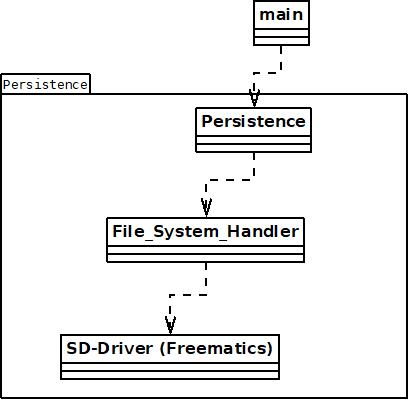
\includegraphics[scale=0.75]{./img/Persistence.jpg}
    \caption{Hierarchie beim SD Zugriff}
    \label{fig:Persistence}
  \end{center}
\end{figure}
Die Aufteilung in die oben gezeigten Klassen hat aber nicht nur eine bessere Lesbarkeit zu Folge. Ein weiterer Vorteil ist auch, eine bessere Trennung der Funktionalitäten voneinander. Den zwei Klassen \texttt{Persistence} und \texttt{File\_System\_Handler} sind folgende Aufgaben zugeteilt:\pagebreak
\subsubsection*{File\_System\_Handler Klasse}
Wie in Abbildung \ref{fig:Persistence} zu sehen ist, greift diese Klasse direkt auf den SD-Kartentreiber zu. Der \texttt{File\_System\_Handler} bietet die Möglichkeit mit von außen aufrufbaren Funktionen Dateien zu erstellen, zu öffnen, zu löschen und anzulegen. Diese Klasse sollte im Gesamtsystem nur einmal vorkommen, da sie eine Menge an Speicherplatz benötigt und der RAM auf dem \textit{ATmega328p} auf 2KB beschränkt ist.\cite{Atmega328P} Die Implementierung eines Singelton Patterns erfolgte nicht um zusätzlich benötigten Speicherplatz zu vermeiden.
Des weiteren ist es pro File\_System\_Handler nur möglich eine einzige Datei zu öffnen und nicht mehrere auf einmal. Auch das ist eine Schutzmaßname um unnötige Speicherplatz Verschwendung zu verhindern.
\subsubsection*{Persistence Klasse}
Da die erstellten Log-Dateien immer nach einem bestimmten Schema aufgebaut sind, kapselt die Klasse \texttt{Persistence} den \texttt{File\_System\_Handler} in sich. Um Daten zu schreiben erfolgt der Zugriff also immer über die Persistence Klasse und nicht über den \texttt{File\_System\_Handler} selbst. Dieser Mechanismus stellt sicher, dass die erstellten Log-Dateien immer den selben Format entsprechen. Einheitlich formatierte Dateien stellen sicher, dass eine Verarbeitung der geloggten Daten von den anderen Elementen des Systems, wie Backend und App, immer möglich ist.
\subsubsection*{Logging Format}
Wie im obigen Abschnitt bereits erwähnt zeichnen sich gute Log-Dateien durch ein einheitliches Format aus. Doch nicht nur eine einheitliche Formatierung spielt beim SmartCar eine Rolle, sondern auch der Speicherbedarf. So muss bei der Erfassung der Daten in einem kompakter Format erfolgen. Dieses Anforderung folgt schon alleine aus der Tatsache, dass es möglich sein soll, die geloggten Daten von dem Dongle über Bluetooth Low Energy(BLE) zu übertragen. Wären die Daten übermäßig groß, müsste ein Nutzer lange Zeit für den Transfer der Daten warten, was die Nutzbarkeit dieses Features beeinträchtigen würde. Aus diesen Gründen wurde das Datenformat aus Abbildung \ref{fig:LoggingEntry} für das Logging gewählt:
\begin{figure}[h]
\begin{center}
  \begin{tabular}{ | c || c | c | c | c |}
    \hline
    \textbf{Byte} & 1. & 2. - 9. & 10. - 11. & 12. - 15. \\ \hline
    \textbf{Wert} & MVID & Datum(ms) & Daten ID & Datenwert \\
    \hline
  \end{tabular}
  \caption{Format eines Logging Eintrags auf der SD-Karte (15Byte)}
  \label{fig:LoggingEntry}
\end{center}
\end{figure}
\subsubsection*{MVID}
Das erste Byte des Eintrags beschreibt die gemappte Fahrzeugnummer. Dieser Eintrag ist wichtig um die bei Verwendung des Dongles in mehreren Fahrzeugen die einzelnen Fahrzeuge und die einzelnen Routen auseinander zu halten. MVID ist eine fortlaufende Nummer von 0 bis 255 die bei jedem Einschalten des Fahrzeugs um eine Stelle erhöht wird. Die definierten 8 Bit stellen einen ausreichenden Zahlenraum dar, um ein komfortables Fahrtenmanagement zu gewährleisten. 
\subsubsection*{Datum}
Die nächsten 8 Byte beinhalten den Zeitstempel des Erfassten Wertes. Dieser wird in Millisekunden seit 01. Januar 1970 angegeben. Die Zeit ist einer der wichtigsten Werte für das Loggen, da nur so bei späteren Analysen festgestellt werden kann wann der Wert aufgenommen wurde. Der Zahlenbereich wurde auf 64 Bit festgelegt, da ein 32-Bit Wert nur bis ungefähr 2038 zählen könnte. Mit 64 Bit lässt sich ein weitaus größerer Zeitraum abdecken.
\subsubsection*{Daten ID}
Der 3. Wert is die ID des geloggtem Datums und liegt im 10. und 11. Byte. Dieser Wert richtet sich nach der in Abschnitt \ref{sec:systemDesign} gezeigten OBD-Tabelle. Zusätzlich zu den OBD-IDs kann dieses Feld Werte für die GPS-Koordinaten, den Beschleunigungssensor und das Gyroskop annehmen.  Nur mit der zugehörigem ID kann dem Wert eine Bedeutung zugeteilt werden. 
\subsubsection*{Wert}
Die letzten 4 Bytes des Eintrags beinhalten den eigentlichen erfassten Wert. Je nach ID muss dieser Wert anders interpretiert werden.
\subsection{Bluetooth Kommunikation}
\label{sec:Bluetooth}
Wie dem Kapitel \ref{sec:useCases} besteht die Möglichkeit mit dem Dongle über Bluetooth mit einer Smartphone App zu kommunizieren. Hierfür wird der Freematics ONE mit dem Bluetooth Low energy fähigem CC2541 Modul von Texas Instruments ausgeliefert.
\begin{figure}[h]
  \begin{center}
    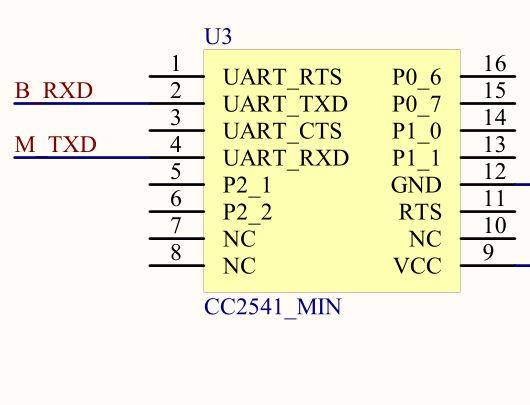
\includegraphics[scale=0.5]{./img/BLEChip.jpg}
    \caption{Schematischer Aufbau des CC2541 Quelle: \url{https://freematics.com/dl/Freematics_ONE_schematic_print_2016.pdf}}
    \label{fig:BLEChip}
  \end{center}
\end{figure} 
Abbildung \ref{fig:BLEChip} zeigt den schematischen Aufbau des Chips und seine PINs. Die zwei UART Pins des Chips(UART\_TXD/UART\_RXD) sind mit den UART Pins des ATmega328p(B\_RXD/M\_TXD) verbunden. Der CC2541 ist so konfiguriert, dass jede Nachricht die von dem Mikrocontroller über UART versendet wird direkt über Bluetooth nach Außen gesendet wird. Dadurch entsteht der Effekt, dass für Nachrichten, die über die der Dongle über die Arudino Funktion \texttt{Serial.println()} ausgibt, automatisch ein Versenden über BLE erfolgt.
\paragraph{}{}
Aus diesem Grund gibt es beim SmartCar Code keine eigene Driver Schicht für die Bluetooth Kommunikation, denn diese ist bereits in den Arduino Bibliotheken implementiert. Der Dongle nutzt Bluetooth um die folgenden 2 Funktionen auszuführen.
\subsubsection*{1. Live Daten Übertragung}
Um Verschiedene Daten der OBD Schnittstelle während der Fahrt zu visualisieren besteht eine Verbindung der APP mit dem Dongle über Bluetooth. Der Dongle sendet bestimmte Daten nach dem Auslesen über Bluetooth zur App.
\begin{figure}[h]
\begin{center}
  \begin{tabular}{ | c | c | c | c | c |}
    \hline
    Startzeichen & ID & Trennzeichen & Wert & Endzeichen \\ \hline
    \# & uint16 & : & uint32 & ; \\
    \hline
  \end{tabular}
  \caption{Format einer Livedaten Nachricht}
  \label{fig:LiveDataMessage}
\end{center}
\end{figure}
Eine Live Daten Nachricht, wie in Abbildung \ref{fig:LiveDataMessage} zu sehen gliedert sich in folgende Teile:
\begin{enumerate}
  \item Start der Nachricht\textbf{(\#)}: Eine Raute am Anfang der Nachricht signalisiert, dass es sich bei dieser Nachricht um eine Live-Daten Nachricht handelt. Dieses Markieren verhindert ein versehentliches interpretieren eine anderen Nachricht als Live-Daten Nachricht.
  \item Daten ID: Direkt nach der Raute folgt die ID des Wertes der in der in der Nachricht enthalten ist. Sie richtet sich wieder nach den OBD-IDs aus Abschnitt \ref{sec:systemDesign}
  \item Trennzeichen(\textbf{:}): Nach der ID kommt ein Doppelpunkt als Trennzeichen
  \item Wert mit \textbf{;} am Ende: Als letztes enthält die Nachricht der Wert zur ID gefolgt von einem Strichpunkt und einem Zeilenumbruch 
\end{enumerate}
\pagebreak
\subsubsection*{2. Upload der Logdateien}
Die zweite Funktion des Dongles, die Bluetooth benötigt ist der Upload der geloggten Daten zum Smartphone. Der Dongle sendet hier nach einem Signal des Smartphones auf Nutzerwunsch Daten von der SD-Karte zur App. Dieses verfahren ist ein zweiter Weg um die Daten vom Dongle ins Backend zur Analyse zu befördern. Das Diagramm in Abbildung \ref{fig:DataUpload} zeigt den Ablauf einer solchen Datenübertragung zwischen App und Dongle. 
\begin{figure}[h]
  \begin{center}
    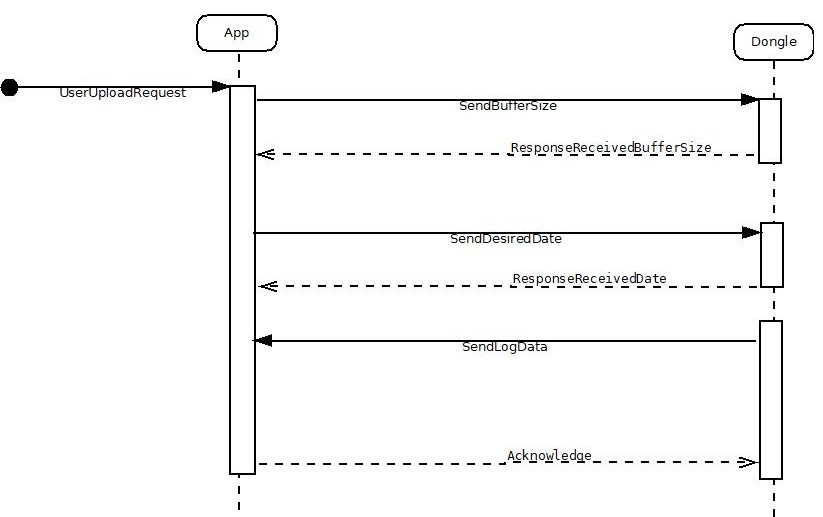
\includegraphics[scale=0.6]{./img/DataUploadSequence.jpg}
    \caption{Ablauf des Datenuploads via Bluetooth}
    \label{fig:DataUpload}
  \end{center}
\end{figure}

Der Ablauf lässt sich in 4 Teile unterteilen:
\begin{enumerate}
  \item Nutzer Request: Der Vorgang des Datenübertragens erfolgt mit der Interaktion des Nutzers auf dem Smartphone. 
  \item Übertragen der Puffer Größe: Nach der Anfrage des Nutzers sendet die App eine Puffer Größe an den Dongle. Diese Zahl stellt die Maximale Anzahl an Logeinträgen dar, die gesendet werden sollen. Diese Nachricht beginnt mit zwei Raute Zeichen(ASCII) gefolgt von einem 8-Bit Wert für den Puffer. Der Dongle bestätigt den Empfang des Puffers mit dem Zurücksenden der gleichen Nachricht. So kann die App sicherstellen, dass für die Pufferübertragung kein Fehler passiert ist. Für eine Puffergröße von 55 würde die Nachricht als String folgendermaßen aussehen: \#\#7 (7 $\equiv$ ASCII 55)
  \item  Mitteilen des Datums: Nach dem Empfang der Antwort des Dongles sendet die App dann das Datum zu dem die Daten übertragen werden sollen. Hier beginnt die Nachricht mit zwei Stichpunkten(ASCII) gefolgt von dem Datum(ASCII) im Format DDMMYYYY. Nach Empfang der Nachricht antwortet der Dongle wie bei der Puffergröße mit der gleichen Nachricht. Für den 01. Januar 2017 wäre die Nachricht ;;01012017
  \item Datenübertragung: Nach dem Austausch der nötigen Informationen beginnt der Dongle mit dem Senden der Daten bis die in 1. definierte Pufffergröße erreicht wurde, oder keine Logdaten mehr vorhanden sind.
\end{enumerate}
